% RUDRA -- Single-image SDR to HDR: bounds, and a gate that reaches one of them.
%
% Build:   bash build.sh          (pdflatex, bibtex, pdflatex, pdflatex)
% arXiv:   bash mkarxiv.sh        (flat package with main.bbl)
%
% The LaTeX is the source of this paper. There is no markdown master: equations,
% numbered floats and cross-references have no faithful markdown form, and the
% generated-from-markdown version this replaced had none of them.
\documentclass[11pt]{article}

\usepackage[utf8]{inputenc}
\usepackage[T1]{fontenc}
\usepackage{lmodern}
\usepackage[margin=1in]{geometry}
\usepackage{microtype}
\usepackage{amsmath,amssymb,textcomp}
\usepackage{bm}
\usepackage{booktabs,array,multirow}
\usepackage{graphicx}
\usepackage[font=small,labelfont=bf]{caption}
\usepackage{siunitx}
\usepackage[numbers,sort&compress]{natbib}
\usepackage[hidelinks]{hyperref}
\usepackage[capitalise,nameinlink]{cleveref}
\usepackage{xcolor}
\usepackage{fancyvrb}
\usepackage{upquote}

\graphicspath{{../docs/figures/}{./figures/}{./}}

\sisetup{group-separator={,}, group-minimum-digits=4, group-digits=integer,
         detect-weight=true, detect-family=true}

% Notation used throughout; defined once so the symbols cannot drift.
\newcommand{\Lsc}{L}                 % scene radiance, cd/m^2
\newcommand{\sdr}{s}                 % 8-bit SDR frame in [0,1]
\newcommand{\base}{b}                % analytic inverse-tone-map baseline
\newcommand{\pred}{\hat{\Lsc}}       % reconstruction
\newcommand{\resid}{r}               % learned log-domain residual
\newcommand{\gate}{g}                % per-pixel residual gate
\newcommand{\hmask}{m_{\mathrm{h}}}  % learned highlight mask
\newcommand{\smask}{m_{\mathrm{s}}}  % learned shadow mask
\newcommand{\sw}{w}                  % per-frame shadow-gate weight
\newcommand{\lscale}{\kappa}         % log_scale = 16
\newcommand{\maxhdr}{L_{\max}}       % network ceiling, 4.0 = 40,000 nits
\newcommand{\nits}{\ensuremath{\mathrm{cd/m^2}}}

\title{What an 8-Bit Frame Can and Cannot Say About the Scene Behind It\\[0.4em]
\large Bounds for single-image inverse tone mapping, and a gate that reaches one of them}

\author{Ahmed Abdelnaby$^{1}$ \qquad Ahmed Talaat$^{1}$ \\[0.35em]
\normalsize $^{1}$FXTD Studios, Cairo, Egypt}
\date{11 September 2026}

\begin{document}
\maketitle

\begin{abstract}
We treat single-image inverse tone mapping as a question about information
rather than about model capacity. A compact residual model on an analytic
inverse tone map is scored against that same analytic map on 429 held-out
frames, in PU21-PSNR and in ColorVideoVDP (CVVDP) JOD. On degraded input, the
condition in which real footage arrives, it gains \SI{1.43}{\decibel} and
\num{0.44}~JOD and wins 348 of 429 frames. On clean, well-graded input it loses
\SI{3.0}{\decibel} of PU21-PSNR for a perceptually invisible $-0.046$~JOD, the two metrics
disagreeing sharply about the practical significance of the same difference,
which is itself one of our results. The regression is not diffuse: it is carried by
low-dynamic-range frames, and the model has no representation of how much
headroom a frame has, so it cannot decide to do nothing.

We then measure what repairing that is worth and whether it can be repaired. An
oracle per-frame scale on the residual is worth \SI{+5.84}{\decibel} on clean
and \SI{+0.29}{\decibel} on degraded input at the same time, and no constant
achieves it. But a linear readout of the features such a gate would see explains
\num{3}\% of that scale's variance, and \num{79}\% of the variance lies within a
condition rather than between conditions, so even a perfect
clean-versus-degraded classifier is capped at $R^2 = \num{0.213}$. The residual
variance asks whether a clipped region was a \SI{200}{\nits} lamp or a
\SI{20000}{\nits} sun. Capacity, corpus and objective were each varied by a
factor of four to six and none of them moved the result. We report this as an
empirical identifiability bound on the representations we tested, not as an
information-theoretic one.

That bound is a property of the question. Posed as a continuous per-frame scale
it is unreachable; posed as a binary decision on the one axis that is
detectable, it is reachable. A \num{21121}-parameter gate on the shadow arm of
the reconstruction converts the clean regression into a gain of
$+3.41 \pm 0.32$~dB and $+0.135 \pm 0.023$~JOD over the shipped model,
for $0.30 \pm 0.15$~dB and $0.091 \pm 0.041$~JOD given up on degraded
input, across three seeds.

\end{abstract}

\section{Introduction}
\label{sec:introduction}

An 8-bit delivery frame is the end of a lossy chain. Scene radiance spanning
perhaps twenty stops was metered, exposed, graded through a tone curve chosen by
a colourist, clipped at both ends and quantised to 256 levels per channel.
Single-image inverse tone mapping asks for the radiance back. The task is
attractive because the input is abundant and the output is what every high
dynamic range (HDR) pipeline needs, and it is hard for a reason that is easy to
state and easy to forget: the forward map is not injective, and no amount of
model does anything about that.

The literature has largely treated the problem as one of architecture and
training. We treat it as one of information, and the distinction turns out to be
load-bearing. This paper reports a compact model, the conditions under which it
helps and hurts, a measurement of the ceiling on adapting it per frame, and a
component that reaches a particular part of that ceiling by asking a different
question of the same input.

\paragraph{Position of this work.}
Our model is deliberately small (\num{1196197} parameters) and is a residual on
an analytic inverse tone map rather than a direct predictor. That choice is what
makes the paper's central question askable at every point in training and
evaluation: \emph{does the network beat doing nothing?} A direct predictor has
no ``nothing'' to be compared against, and in practice a great deal of what a
learned inverse tone mapper appears to contribute is recoverable analytically.
Every number in this paper is a difference against that analytic baseline on
identical inputs.

\paragraph{Contributions.}
\begin{enumerate}
\item \textbf{A conditional characterisation of when learned inverse tone
  mapping helps.} On degraded input the model gains \SI{1.43}{\decibel}
  PU21-PSNR and \num{0.44}~JOD over the analytic baseline, on 81\% of held-out
  frames. On clean input it loses \SI{3.0}{\decibel} PU21-PSNR for
  $-0.046$~JOD. Reporting either condition alone misrepresents the method
  (\cref{sec:results}).

\item \textbf{A characterised disagreement between the two standard HDR
  metrics.} On the same frames and the same models, PU21-PSNR reports a
  substantial fidelity penalty where CVVDP reports a perceptually negligible
  difference, and the two agree decisively when the difference is large. The
  two are not commensurable as numbers, which is the point: what differs is the
  practical significance each assigns to a small reconstruction difference on
  well-graded input. We localise that divergence, show it is only partly carried
  by the error tail, and show it reappearing inside a checkpoint-selection rule
  that touches neither metric
  (\cref{sec:results,sec:failure,sec:methodology}).

\item \textbf{A localisation of the failure to a specific mechanism.} The clean
  regression is not invented highlights, which was our own first two hypotheses.
  It is the shadow arm of the residual gate firing on scenes that need no
  reconstruction, and disabling that arm inverts the regression
  (\cref{sec:failure}).

\item \textbf{A measured bound on per-frame adaptation.} An oracle per-frame
  residual scale is worth \SI{+5.84}{\decibel} on clean and
  \SI{+0.29}{\decibel} on degraded input simultaneously, and is poorly
  identifiable from the input we have: a linear readout of the features the gate
  sees explains \num{3}\% of its variance, and \num{79}\% of the variance lies
  within a condition rather than between, which caps \emph{any}
  condition-detection architecture at $R^2 = \num{0.213}$ regardless of how it
  is built. Capacity, corpus and objective were each varied by a factor of four
  to six without moving it. We are careful to claim an empirical identifiability
  result and not an information-theoretic one; \cref{sec:bound} separates what
  the measurements establish from what they suggest.

\item \textbf{A component that reaches the reachable part of that bound.} Posed
  as a binary decision on the detectable axis rather than as a continuous scale,
  the problem is tractable. A \num{21121}-parameter gate on the shadow arm
  delivers $+3.41 \pm 0.32$~dB and $+0.135 \pm 0.023$~JOD on clean input
  for $0.30 \pm 0.15$~dB and $0.091 \pm 0.041$~JOD on degraded input
  across three seeds, and is the only configuration we scored that is positive
  on all four measures (\cref{sec:gate}).

\item \textbf{Three defects in our own evaluation harness, reported rather than
  quietly repaired.} Checkpoint selection on the maximum of a noisy series, an
  evaluation that silently read the alphabetical front of its split, and a
  viewer that presented every frame upside down beneath tests that compared only
  float buffers. Each corrupted a result we believed, and each is available to
  any comparable pipeline (\cref{sec:methodology}).
\end{enumerate}

\paragraph{Scope.}
This paper reports a direct SDR-pixel to scene-linear-radiance image model. It
does not report the DRE-transformer and cross-attention architecture described
in an earlier manuscript from this group: that design was never trained, and the
results attributed to it were aspirational. Both are withdrawn.
\Cref{sec:withdrawal} states what was withdrawn and why, so that a reader who
has seen the earlier document can reconcile the two. What follows is the system
that exists, measured with the metrics that exist.

\section{Related work}
\label{sec:related}

\paragraph{A note on how these references are used.}
Every reference below was checked against the publisher or author page for
authors, title, venue and year, and the one-line method descriptions are at the
level the titles and abstracts support. No number in this paper is attributed to
any of them. We compare against our own analytic baseline and against ExpandNet
run from its authors' released weights (\cref{sec:expandnet});
\cref{sec:limitations} states which comparisons are still missing. The failure
mode this caution replaces, placeholder tables presented as measurements, is
documented in \cref{sec:withdrawal}.

\paragraph{Single-image inverse tone mapping.}
The dominant framing learns a mapping from an 8-bit frame to a higher-range one,
typically with an encoder-decoder and a loss in a perceptual or log domain, and
typically evaluated on synthetically clipped data. Eilertsen et
al.~\citep{eilertsen2017} predict a log-domain reconstruction of the saturated
regions with a U-Net and blend it back through a saturation mask; Marnerides et
al.~\citep{marnerides2018} combine three branches at different receptive fields;
Endo et al.~\citep{endo2017} instead synthesise a bracketed exposure stack from
the single input and merge it; Liu et al.~\citep{liu2020} decompose the task into
learned inverses of the individual camera-pipeline stages. Our architecture is
deliberately smaller than this line of work and is a residual on an analytic
inverse tone map rather than a direct predictor, which is what makes ``does the
network beat doing nothing?'' a question we can ask at every step of training.

\paragraph{Highlight and clipped-region reconstruction.}
A related family treats the problem as inpainting the saturated regions
specifically, rather than remapping the whole frame. Santos et
al.~\citep{santos2020} make the clipped area explicit by masking it out of the
network's own features and adding a perceptual loss, and the masked blend of
Eilertsen et al.~\citep{eilertsen2017} serves the same end. Our highlight and
shadow masks share that purpose but are predicted jointly with the residual and
gated by a luminance prior rather than by a detected saturation mask.
\Cref{sec:failure} is a direct criticism of that choice: our own failures are
not in the clipped highlights at all.

\paragraph{Evaluation of HDR reconstruction.}
PU21 \citep{pu21} and ColorVideoVDP \citep{cvvdp} are the two public measuring
sticks we use, the first an encoding that makes existing metrics such as PSNR
applicable to absolute-luminance HDR, the second a calibrated visible-difference
predictor reporting in JOD. \Cref{sec:results} reports a case where they diverge sharply in the practical
significance they assign to the same difference on the same frames, and
\cref{sec:failure} shows the PU21 penalty is only partly tail-carried. We are
not aware of that disagreement having been characterised for this task, and
consider it a contribution independent of the model.

\paragraph{Training data for HDR.}
The scarcity of paired SDR/HDR footage shapes every result here. Public HDR
video with cinematic production values remains small enough to enumerate: the
HDM-HDR-2014 set of Froehlich et al.~\citep{froehlich2014} contributes 9 scenes
and \num{11007} frames to our corpus, and the widely used HDR still sets
\citep{kalantari2017} are bracketed-exposure captures rather than graded footage.
The remainder of our corpus is proprietary. \Cref{sec:corpus} documents a
distribution shift between our own training and held-out splits that we did not
design and that a reader should weigh.

\paragraph{What we compare against.}
ExpandNet \citep{marnerides2018} is scored on our split in \cref{sec:expandnet},
using the authors' own model and released weights and their own pre- and
post-processing. Our benchmark harness scores any third-party output against the
same reference, so the remaining comparisons are a matter of running published
code rather than of building anything; \cref{sec:limitations} says which are
outstanding.

\section{Problem formulation}
\label{sec:formulation}

\subsection{Units and storage}
\label{sec:units}

Absolute units are not a presentation detail in this problem; conflating two
conventions is a multi-stop error that produces entirely plausible numbers. We
therefore fix them once. HDR targets are stored in a \texttt{log2\_extended}
encoding covering \SI{0.005}{\nits} to \SI{1000000}{\nits} at \num{2377} codes
per stop. \emph{Network units} are \si{\nits} divided by \num{10000}, so
$\Lsc = 1.0$ denotes \SI{10000}{\nits} and diffuse white, taken at
\SI{203}{\nits} after ITU-R BT.2408 \citep{bt2408}, is $\Lsc = \num{0.0203}$.
The network clamps its output at $\maxhdr = 4.0$, that is \SI{40000}{\nits}.
Storage elsewhere in the pipeline uses the delivery convention in which $1.0$ is
diffuse white; the two differ by a factor of \num{49.26} and are never mixed
within a computation.

\subsection{The forward map, and where it is not invertible}
\label{sec:forward}

Let $\Lsc \in \mathbb{R}^{H \times W \times 3}_{\ge 0}$ be scene radiance in
network units. An 8-bit delivery frame $\sdr \in [0,1]^{H \times W \times 3}$ is
produced by
\begin{equation}
\sdr \;=\; Q_{8}\!\left(\operatorname{clip}_{[0,1]}\big(T(\Lsc)\big)\right),
\label{eq:forward}
\end{equation}
where $T$ is a display-referred transform, in general an unknown composition of
exposure, a creative grade and a tone curve; $\operatorname{clip}$ is the
delivery range limit; and $Q_{8}$ is quantisation to 256 levels per channel.

Two distinct failures of injectivity follow, and the distinction matters for
everything after \cref{sec:results}. Where $T(\Lsc) \ge 1$ the frame is
\emph{clipped}: all radiances above the clipping point share one code.
Where $T(\Lsc)$ falls below the first few codes the frame is \emph{crushed}: a
range of low radiances shares a small number of codes, and quantisation noise
there is large relative to the signal. Inverting \cref{eq:forward} exactly is
possible only on the interior, where $T$ is monotone and the quantisation step
is small relative to the local slope.

\subsection{Censored observations}
\label{sec:censoring}

Graded HDR sources carry a delivery ceiling $c$: \SI{4000}{\nits} for
HDM-HDR-2014, approximately \SI{1000}{\nits} for Rec.2100 PQ 1K,
\SI{10000}{\nits} for Chimera. A target pixel sitting on that ceiling states
$\Lsc \ge c$, not $\Lsc = c$. Treating it as an equality trains the model to cap
its own highlights, which is the specific failure the ceiling-aware loss exists
to prevent, and 78\% of the image corpus and 84\% of the video corpus are graded
to such a ceiling.

We therefore treat those pixels as right-censored observations. Writing
$\ell(x) = \log(1 + \lscale x)$ for the log-radiance encoding with
$\lscale = 16$, the per-pixel error is
\begin{equation}
e \;=\;
\begin{cases}
\big[\ell(\Lsc) - \ell(\pred)\big]_{+} \;+\; \big[\ell(\pred) - \ell\big(\min(2^{3}c,\, 10^{6})\big)\big]_{+}
  & \text{if } \Lsc \ge c(1 - 10^{-3}),\\[4pt]
\big|\,\ell(\pred) - \ell(\Lsc)\,\big| & \text{otherwise,}
\end{cases}
\label{eq:censored}
\end{equation}
with $[\,\cdot\,]_{+} = \max(0, \cdot)$. Under-prediction of a censored pixel is
charged; over-prediction is free for
$\texttt{CENSORED\_HEADROOM\_STOPS} = 3$ stops above the ceiling and charged
beyond. Without that second term a purely one-sided loss has no upper anchor and
the cheapest behaviour for a censored pixel is to run to $\maxhdr$. Three stops
takes a \SI{4000}{\nits} graded clip to \SI{32000}{\nits}, which covers real
specular highlights without licensing invention. The $10^{-3}$ relative slack
absorbs a \texttt{uint16} log round trip in the stored target.

Censoring is a small effect on the evaluation corpus even though it shapes
training: the mean censored fraction is \num{0.0003}.

\subsection{What ``reconstruction'' can and cannot mean here}
\label{sec:claim}

Given \cref{eq:forward}, a method that maps $\sdr$ to $\pred$ is not recovering
$\Lsc$ on the clipped set; it is estimating a plausible value consistent with
the observation $\Lsc \ge c$. On the interior it is inverting a transform, which
is a different and far better-posed operation. The results in
\cref{sec:results,sec:bound} are best read with that split in mind: the analytic
baseline is strong precisely because most pixels of most frames are interior,
and the learned component earns its place where they are not.

\section{Method}
\label{sec:method}

\subsection{Analytic baseline}
\label{sec:baseline}

The baseline is an analytic inverse of the transform used to render the corpus
SDR side,
\begin{equation}
\base(\sdr) \;=\; \operatorname{ACES}^{-1}\!\big(\operatorname{sRGB}^{-1}(\sdr)\big)
\cdot \frac{2 \cdot 203}{\num{10000}},
\label{eq:baseline}
\end{equation}
in network units. The factor $203/\num{10000}$ places diffuse white, and the
factor $2$ is the \SI{-1}{EV} the corpus preparation applies before the ACES
curve. \Cref{eq:baseline} is therefore \emph{exact} for corpus frames and
approximate for SDR produced by any other pipeline, which is a property of the
baseline and not of the model; the learned component is what absorbs other
camera and tone curves. Every comparison in this paper is against
\cref{eq:baseline} on identical inputs, so the exposure convention cancels.

\subsection{Composite}
\label{sec:composite}

A compact U-Net $f_\theta$ (\num{1196197} parameters, \SI{4.6}{MiB} in float32)
takes the SDR frame and its baseline and predicts three fields: a log-domain
residual $\resid$, a highlight mask $\hmask$ and a shadow mask $\smask$. Let
$y = \operatorname{luma}(\sdr)$ be Rec.709 luma of the SDR frame. The residual is
applied through a fixed per-pixel prior
\begin{align}
p_{\mathrm{h}} &= \sigma\big(24\,(y - 0.82)\big), &
p_{\mathrm{s}} &= \sigma\big(24\,(0.10 - y)\big), &
\gate &= \max\big(p_{\mathrm{h}},\; \sw \cdot p_{\mathrm{s}}\big),
\label{eq:prior}
\end{align}
where $\sw \in [0,1]$ is a per-frame weight on the shadow arm, fixed at $1$ for
the shipped model and predicted by the gate of \cref{sec:gate}. The composite is
\begin{align}
\ell(\pred) &= \operatorname{clip}_{[0,\;\ell(\maxhdr)]}\Big(\ell\big(\base(\sdr)\big) + \resid \cdot \gate\Big),
\label{eq:composite}\\
\pred &= \ell^{-1}\big(\ell(\pred)\big),
\qquad \ell(x) = \log(1 + \lscale x),\; \lscale = 16 .
\end{align}
Outside the recovery region the baseline is restored explicitly,
\begin{equation}
\pred \;\leftarrow\; \base(\sdr) + \max(\hmask, \smask)\cdot\big(\pred - \base(\sdr)\big),
\label{eq:preserve}
\end{equation}
so that the physically grounded analytic inverse survives through ordinary
midtones and learned capacity is spent where \cref{eq:forward} was not
invertible.

Two properties of \cref{eq:prior} carry the rest of the paper. First, the prior
is a function of \emph{one pixel's brightness and nothing else}: it has no access
to the frame, and therefore no representation of how much headroom the scene
has. \Cref{sec:failure} shows this is the mechanism behind the clean regression.
Second, the two arms are separable, and $\sw = 1$ and $\sw = 0$ reproduce
exactly the two configurations that \cref{sec:ablation} measures, which is what
makes the gate of \cref{sec:gate} an interpolation between measured endpoints
rather than a new model.

\subsection{Training objective}
\label{sec:objective}

Write $e$ for the censored per-pixel error of \cref{eq:censored}, $h$ and $s$
for the ground-truth highlight and shadow masks, and
$\rho = \max(h, s)$ for the recovery region. The objective is
\begin{multline}
\mathcal{L} = \underbrace{\overline{e}}_{\text{log } L_1}
\;+\; 0.50\,\mathcal{L}_{\mathrm{hi}}
\;+\; 0.20\,\mathcal{L}_{\mathrm{sh}}
\;+\; 0.10\,\mathcal{L}_{\mathrm{chroma}}
\;+\; \lambda_{\mathrm{sc}}\,\mathcal{L}_{\mathrm{shadow\text{-}chroma}}
\;+\; \lambda_{\mathrm{ss}}\,\mathcal{L}_{\mathrm{shadow\text{-}smooth}}\\
\;+\; 0.10\,\mathcal{L}_{\mathrm{edge}}
\;+\; 0.05\,\mathcal{L}_{\mathrm{mask}}
\;+\; 0.05\,\mathcal{L}_{\mathrm{outside}}
\;+\; 0.10\,\mathcal{L}_{\mathrm{resid\text{-}outside}},
\label{eq:loss}
\end{multline}
where $\mathcal{L}_{\mathrm{hi}}$ and $\mathcal{L}_{\mathrm{sh}}$ are $e$
averaged over the highlight and shadow masks, $\mathcal{L}_{\mathrm{chroma}}$ is
an $L_1$ on normalised chromaticity, $\mathcal{L}_{\mathrm{shadow\text{-}chroma}}$
is an $L_1$ on opponent channels within the shadow mask (chromaticity ratios are
poorly conditioned near black, where they force legitimate shadows toward
neutral grey), $\mathcal{L}_{\mathrm{shadow\text{-}smooth}}$ penalises residual
gradients inside the shadow mask, $\mathcal{L}_{\mathrm{edge}}$ is a gradient
term on log radiance, $\mathcal{L}_{\mathrm{mask}}$ is binary cross-entropy on
the two predicted masks, and the last two terms charge error and residual
magnitude \emph{outside} $\rho$, which is what holds \cref{eq:preserve} honest
during training. The two $\lambda$ weights are schedule parameters; the
remainder are fixed.

\section{Experimental setup}
\label{sec:setup}

\subsection{Corpus and splits}
\label{sec:corpus}

The corpus holds \num{27678} training, \num{435} validation and \num{429} test
records; validation and test are 97 scenes each at $1280 \times 720$. Sampling is
scene-balanced with 40\% video mass. The only publicly redistributable component
is the HDM-HDR-2014 set of Froehlich et al.~\citep{froehlich2014}, 9 scenes and
\num{11007} frames at a median \num{5.99} stops of measured dynamic range; the
remainder is proprietary footage, which is why \cref{sec:reproducibility} ships
the manifests and the scoring harness rather than the corpus. The manifest is
pinned by SHA-256 in every checkpoint's configuration, so a run can be tied to
the exact record set it saw.

\subsection{An unintended distribution shift}
\label{sec:shift}

The held-out splits are not drawn from the training distribution
(\cref{tab:shift}). The band in which the model fails, below
\SI{400}{\nits}, is 45.2\% of the test split and 27.2\% of what the sampler
draws. We report this because it is a confound in our own results;
\cref{sec:ceiling} argues that it is not the binding constraint, and
\cref{sec:limitations} records that we have not retrained under a matched
sampler to prove that.

\begin{table}[htbp]
\centering
\caption{The held-out splits are lower in dynamic range than the training
distribution the sampler draws from. Peak is the reference peak luminance of the
frame.}
\label{tab:shift}
\begin{tabular}{lrrrr}
\toprule
 & median peak & $<$ \SI{1000}{\nits} & $<$ \SI{400}{\nits} & video share \\
\midrule
train, as sampled & \SI{1713}{\nits} & 42.2\% & \textbf{27.2\%} & 40.0\% \\
validation        & \SI{548}{\nits}  & 69.0\% & 38.2\% & 33.8\% \\
test              & \SI{546}{\nits}  & 58.0\% & \textbf{45.2\%} & 32.9\% \\
\bottomrule
\end{tabular}
\end{table}

\subsection{Training configuration}
\label{sec:training}

\Cref{tab:training} gives the shipped configuration (v5) and the capacity
ablation (v6), which differ only in width. Both were trained on a single NVIDIA
RTX 4080 SUPER.

\begin{table}[htbp]
\centering
\caption{Training configuration. v6 differs from v5 only in base width, and is
the capacity ablation of \cref{sec:capacity}.}
\label{tab:training}
\begin{tabular}{lp{0.44\linewidth}p{0.16\linewidth}}
\toprule
 & v5 (shipped) & v6 (capacity) \\
\midrule
base channels & 32 & 64 \\
parameters & \num{1196197} & \num{4770117} \\
crop & 384 & 384 \\
batch $\times$ grad-accum & $2 \times 2$ & same \\
optimiser & AdamW, lr $2\!\times\!10^{-4}$, wd $10^{-4}$, cosine to 5\% & same \\
gradient clip & 1.0 & same \\
degradation probability & 0.65 & same \\
scene-balanced sampling & yes, 40\% video mass & same \\
steps & \num{100000} & \num{100000} \\
evaluation & every \num{1000} steps, 256 held-out crops, both conditions & same \\
selection & trailing median of \texttt{composite\_gain} (\cref{sec:selection}) & same \\
seed & \num{20260715} & \num{20260715} \\
\bottomrule
\end{tabular}
\end{table}

\subsection{Conditions, metrics and protocol}
\label{sec:protocol}

\paragraph{Conditions.} \textsc{clean} is the held-out frame as prepared, a
well-graded plate. \textsc{hard} applies a seeded camera and codec degradation
to the same frame: an unknown tone curve, 4:2:0 chroma subsampling, banding and
JPEG. \textsc{hard} is the deployment condition; \textsc{clean} is the condition
in which the analytic baseline is already strong.

\paragraph{Reference.} Both conditions are scored against the same
\emph{unclamped} reference. Clamping the reference at the network's own ceiling
would score the model against a ground truth cropped to its own limits, which
flatters it exactly where it is weakest.

\paragraph{Metrics.} PU21-PSNR \citep{pu21} in decibels and ColorVideoVDP
\citep{cvvdp} in JOD, both at \texttt{--nits-scale 203}. A JOD is a
just-noticeable difference unit; differences well below \num{0.1}~JOD are not
expected to be visible. Reporting the two together is not redundancy:
\cref{sec:disagreement} shows they can put a substantial penalty and a
perceptually negligible one on the same comparison. The two are in different
units and are not directly comparable as numbers; what is comparable is whether
each calls a difference significant.

\paragraph{Reported quantity.} Unless stated otherwise, every number is a
\emph{paired difference} against the analytic baseline of \cref{eq:baseline} on
the same frame under the same condition, so corpus difficulty cancels. ``Frames
won'' counts frames on which that paired difference is positive, out of 429.

\paragraph{Statistical protocol.} The headline comparisons are over all 429
held-out frames, paired, and we report the mean and median of the per-frame
difference rather than the difference of means. The oracle and ceiling analyses
of \cref{sec:bound} use one frame per scene (27 and 51 frames respectively) for
cost reasons, and \cref{sec:limitations} quantifies the bias that introduces.
Where a result rests on a margin comparable to run-to-run variation, we retrain
and report mean $\pm$ standard deviation across seeds: \cref{sec:seeds} does
this for the gate with $n = 3$. Three runs support the claim that a sign is
stable; they do not support a confidence interval, and we do not present one.

\section{Results}
\label{sec:results}

\subsection{The model against its own analytic baseline}
\label{sec:headline}

\Cref{tab:headline} gives absolute scores for every configuration on the 429
held-out frames, and \cref{tab:paired} the paired per-frame differences for the
shipped model.

\begin{table}[htbp]
\centering
\caption{Absolute scores on 429 held-out frames. The shipped model (v5) is the
best configuration on degraded input and the worst on clean; only the gated
configuration of \cref{sec:gate} is at or above the analytic baseline on both.}
\label{tab:headline}
\begin{tabular}{llrr}
\toprule
Condition & Method & PU21-PSNR (dB) & CVVDP (JOD) \\
\midrule
clean & analytic baseline            & \textbf{45.99} & 9.448 \\
clean & v5 (32 ch, step \num{81000}) & 42.99 & 9.402 \\
clean & v6 (64 ch)                   & 43.24 & 9.452 \\
clean & \textbf{v5 + shadow gate}    & \textbf{46.06} & \textbf{9.561} \\
\midrule
hard  & analytic baseline            & 25.92 & 7.362 \\
hard  & \textbf{v5}                  & \textbf{27.34} & \textbf{7.805} \\
hard  & v6                           & 26.88 & 7.706 \\
hard  & v5 + shadow gate             & 27.15 & 7.751 \\
\bottomrule
\end{tabular}
\end{table}

\begin{table}[htbp]
\centering
\caption{Paired per-frame difference, v5 against the analytic baseline, 429
frames. The clean PU21 loss of \SI{3.0}{\decibel} corresponds to
$-0.046$~JOD, far below a just-noticeable difference.}
\label{tab:paired}
\begin{tabular}{lrrrrr}
\toprule
 & mean $\Delta$ PU21 & median $\Delta$ & frames won & mean $\Delta$ JOD & median $\Delta$ JOD \\
\midrule
hard  & \textbf{+1.427 dB} & +0.609 & \textbf{348 / 429 (81\%)} & \textbf{+0.443} & +0.134 \\
clean & $-2.999$ dB        & $-2.131$ & 115 / 429 (27\%)        & \textbf{$-0.046$} & $-0.040$ \\
\bottomrule
\end{tabular}
\end{table}

\subsection{Fidelity penalty, perceptual indifference}
\label{sec:disagreement}

\begin{figure}[htbp]
\centering
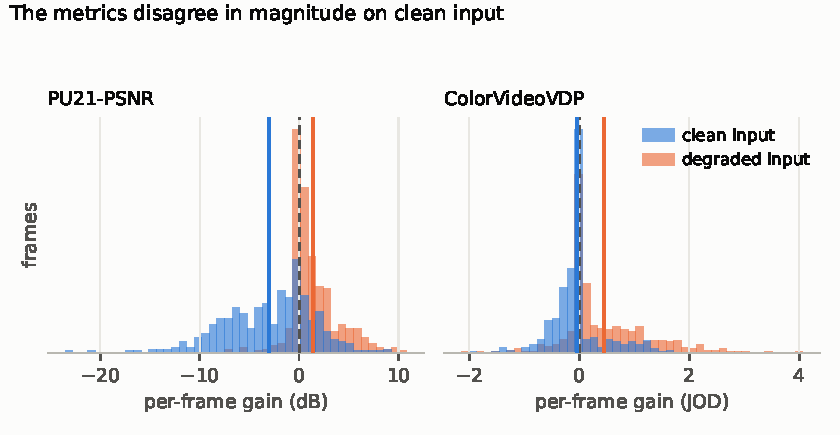
\includegraphics[width=\linewidth]{fig3_metric_disagreement.pdf}
\caption{Per-frame gain over the analytic baseline, 429 held-out frames;
vertical rules mark the means. The clean distribution is broad and left-shifted
in PU21-PSNR and collapses onto zero in CVVDP. The same frames, the same models,
two metrics, one calling the difference substantial and the other calling it
invisible.}
\label{fig:disagreement}
\end{figure}

A \SI{3.0}{\decibel} PU21-PSNR loss corresponds to $-0.046$~JOD
(\cref{fig:disagreement}), far below a just-noticeable difference. What the
model adds to well-graded input is highlight energy that PU21-PSNR punishes and
that no viewer sees. The clean PU21 row should never be reported without the JOD
beside it. \Cref{sec:expandnet} shows the converse case, in which the two agree
decisively, and \cref{sec:selection} shows the disagreement reappearing inside a
selection rule that touches neither metric.

\subsection{A published method on the same split}
\label{sec:expandnet}

Every number above is against our own analytic baseline, which has been this
paper's largest gap since the first draft. It is now closed for one method.
ExpandNet \citep{marnerides2018} was run on the same 429 frames using the
authors' released weights rather than a reimplementation, with their
pre-processing and post-processing unchanged, on the exact 8-bit frames our model
was given (\cref{tab:expandnet}).

\begin{table}[htbp]
\centering
\caption{Clean condition, 429 frames. ExpandNet is \SI{-18.56}{\decibel} and
$-2.029$~JOD against our deployed configuration, winning 1 of 429 frames on
PU21 and 16 on CVVDP.}
\label{tab:expandnet}
\begin{tabular}{lrr}
\toprule
Method (clean, 429 frames) & PU21 (dB) & CVVDP (JOD) \\
\midrule
\textbf{RUDRA + gate, as deployed} & \textbf{46.06} & \textbf{9.561} \\
RUDRA + gate, exposure-aligned     & 46.61 & 9.558 \\
analytic inverse-ACES baseline     & 45.99 & 9.448 \\
v5 backbone, no gate               & 42.99 & 9.402 \\
ExpandNet                          & 27.50 & 7.532 \\
\bottomrule
\end{tabular}
\end{table}

\paragraph{The exposure alignment, and what it is worth to each side.}
ExpandNet ends in a sigmoid and its released post-processing min-max normalises
each frame to $[0,1]$, so it predicts \emph{relative} radiance with no absolute
anchor. Scoring that directly against a reference in \si{\nits} would measure its
exposure guess. We therefore fit one global scalar per frame on the pixels the
SDR input neither clipped nor crushed. That is a free parameter and it is not
free to grant: ExpandNet's fitted scale has a \textbf{$35.5\times$} spread across
frames (p10 \num{0.49}, p90 \num{17.45}), where ours is $1.0\times$ (p10
\num{0.9993}, p90 \num{1.018}) because our model predicts absolute
\si{\nits}. Put through the same fit our model gains \SI{0.55}{\decibel} and
\emph{loses} \num{0.0025}~JOD, so the row we report for ourselves is the
unaligned one.

The alignment is not what costs ExpandNet its score. Given the \emph{best
possible} per-frame exposure, chosen to maximise its own PU21, it recovers
\SI{+0.39}{\decibel}.

\paragraph{Three caveats, because a gap this size invites the question.}
ExpandNet is run outside its training domain: our SDR frames come from an ACES
approximation at a \SI{-1}{EV} offset, not the curve its corpus used. Our
reference is unclamped and reaches roughly a million \si{\nits}, a range no
method trained on display-referred targets was built for. And ExpandNet
compresses dynamic range by a median factor of $2.3\times$ against the reference
where ours is within $1.32\times$, which contributes to but does not explain
\SI{18}{\decibel}. The row should be read as \emph{this method, unmodified, on
this corpus}, not as a ranking of the field. Santos et
al.~\citep{santos2020}, Eilertsen et al.~\citep{eilertsen2017} and Liu et
al.~\citep{liu2020} have public code and have not been run.

\paragraph{What this settles about \cref{sec:disagreement}.}
The two metrics part company on our model against its own baseline and agree
decisively here: \SI{18.6}{\decibel} and \num{2.03}~JOD say the same thing, and
\num{2}~JOD is two just-noticeable differences. The divergence is a property of
\emph{small} differences on well-graded input, not a defect in either
instrument. When the difference is real, both see it.

\subsection{Capacity is not the constraint}
\label{sec:capacity}

v6 quadruples width to \num{4770117} parameters. It is better on clean
(\SI{+0.25}{\decibel}, $+0.05$~JOD) and worse on hard (\SI{-0.46}{\decibel},
$-0.10$~JOD) than v5: movement in both directions, and smaller than the spread
between conditions. \Cref{sec:levers} places this beside the corpus and
objective ablations.

\section{Localising the clean regression}
\label{sec:failure}

\subsection{It is a function of scene headroom}
\label{sec:headroom}

The clean regression is concentrated, not diffuse. Splitting clean frames by the
headroom the ground truth actually has separates them cleanly
(\cref{tab:headroom}), and the trend is monotone across the full range
(\cref{fig:headroom}). The correlation between $\log_2$ of the reference peak
and per-frame gain is $+0.46$.

\begin{table}[htbp]
\centering
\caption{Clean frames split by the headroom of the reference. The model's error
is a function of the scene.}
\label{tab:headroom}
\begin{tabular}{lrr}
\toprule
clean frames & mean $\Delta$ vs baseline & median reference peak \\
\midrule
60 worst & \textbf{\SI{-10.76}{\decibel}} & \SI{238}{\nits} \\
60 best  & \textbf{\SI{+3.41}{\decibel}}  & \SI{19590}{\nits} \\
\bottomrule
\end{tabular}
\end{table}

\begin{figure}[htbp]
\centering
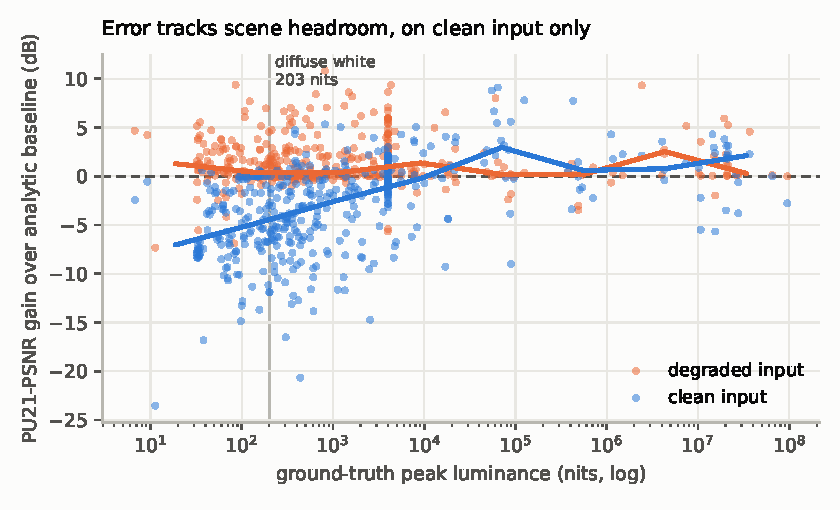
\includegraphics[width=\linewidth]{fig1_gain_vs_headroom.pdf}
\caption{Per-frame gain against reference headroom, log $x$-axis, with binned
medians. On clean input the trend rises through zero at roughly
\SI{10000}{\nits}; on degraded input it is flat and positive at every headroom.}
\label{fig:headroom}
\end{figure}

The mechanism is \cref{eq:prior}. The per-pixel luminance prior cannot
distinguish a \SI{238}{\nits} studio interior from a \SI{20000}{\nits} sunset,
because it never sees the frame.

\subsection{The error is in the shadows, and only partly in the tail}
\label{sec:tail}

On 51 clean held-out frames we computed the per-pixel PU21 squared error for
both the model and the baseline, then recomputed each PSNR with the worst pixels
progressively discarded (\cref{tab:trim}). If the penalty were carried by a few
bad pixels the gap would close.

\begin{table}[htbp]
\centering
\caption{Trimmed PU21-PSNR on clean frames below \SI{400}{\nits}, $n = 25$.
Discarding a tenth of every frame removes \SI{2.3}{\decibel} of the
\SI{5.55}{\decibel} gap and leaves \SI{3.2}{\decibel}: the penalty is partly
tail-carried and mostly broad.}
\label{tab:trim}
\begin{tabular}{lrrr}
\toprule
discard worst & baseline & RUDRA & gap \\
\midrule
---     & 54.40 & 48.84 & \textbf{\SI{-5.55}{\decibel}} \\
0.1\%   & 54.70 & 49.40 & $-5.30$ \\
1\%     & 55.36 & 51.14 & $-4.23$ \\
10\%    & 57.58 & 54.34 & \textbf{\SI{-3.23}{\decibel}} \\
\bottomrule
\end{tabular}
\end{table}

The worst 1\% of pixels carry 32\% of the model's total squared error, but the
bulk of the distribution is genuinely worse too. At those worst pixels the
\emph{true} luminance has median \SI{4}{\nits} against \SI{21}{\nits}
frame-wide: they are darker than typical, not brighter, and only 46\% of them
are over-predicted. On frames at or above \SI{400}{\nits} the model and the
baseline are level (\SI{-0.03}{\decibel}) and the worst pixels move to the
bright end instead (median \SI{560}{\nits} against \SI{57}{\nits} frame-wide).

This relocates the failure. \Cref{eq:prior} has two arms, and on a
low-dynamic-range scene the shadow arm fires on content that needs no
reconstruction at all. The headroom correlation of $+0.46$ is real, but the
mechanism behind it is the \emph{shadow} path, not invented highlights. That is
a specific and testable target, and one that the single global scale of
\cref{sec:bound} could not have isolated.

\subsection{The shadow arm, ablated}
\label{sec:ablation}

The hypothesis is directly testable: disable the shadow prior, setting $\sw = 0$
in \cref{eq:prior}, and rescore the same 429 frames (\cref{tab:ablation}).

\begin{table}[htbp]
\centering
\caption{Gain over the analytic baseline with the shadow arm on and off, 429
frames. Turning it off does not shrink the clean regression, it inverts it.}
\label{tab:ablation}
\begin{tabular}{lrrrr}
\toprule
 & \multicolumn{2}{c}{clean} & \multicolumn{2}{c}{hard} \\
\cmidrule(lr){2-3}\cmidrule(lr){4-5}
configuration & dB & JOD & dB & JOD \\
\midrule
shadow arm \textbf{on} (shipped) & \textbf{$-3.00$} & $-0.046$ & \textbf{$+1.43$} & $+0.443$ \\
shadow arm \textbf{off}          & \textbf{$+0.51$} & $-0.017$ & $+0.33$ & $+0.134$ \\
\bottomrule
\end{tabular}
\end{table}

The hypothesis is confirmed, and the result is a trade rather than a free win.
Turning the shadow arm off moves clean by \SI{+3.51}{\decibel}, so the model now
beats the analytic baseline on clean input by \SI{0.51}{\decibel}, and costs
\SI{1.10}{\decibel} on degraded input. The shadow path is therefore the whole of
the clean regression and simultaneously carries most of the degraded-input gain,
which is what one would expect: crushed shadows are exactly what a bad tone
curve produces and exactly what a well-graded frame does not have.

This is the observation that makes \cref{sec:gate} possible, and
\cref{sec:bound} is what makes it necessary to state the problem that way.

\section{A bound on per-frame adaptation}
\label{sec:bound}

\subsection{What an oracle gate is worth}
\label{sec:oracle}

Give the composite a single global scale $\alpha$ on the residual, so that
$\gate \leftarrow \alpha\,\gate$ in \cref{eq:composite}, and let an oracle choose
it per frame (\cref{tab:alpha}, 27 held-out scenes).

\begin{table}[htbp]
\centering
\caption{PU21 gain over the analytic baseline as a function of a global residual
scale $\alpha$, 27 held-out scenes. Per-frame adaptation beats the shipped
configuration on both conditions at once, which is not a trade-off at all.}
\label{tab:alpha}
\begin{tabular}{lrr}
\toprule
$\alpha$ & clean & hard \\
\midrule
$1.0$, as shipped           & \textbf{$-4.15$} & $+1.08$ \\
$0.125$, best single constant & $+0.83$ & \textbf{$+0.17$} \\
per-frame oracle            & \textbf{$+1.69$} & \textbf{$+1.37$} \\
\bottomrule
\end{tabular}
\end{table}

\begin{figure}[htbp]
\centering
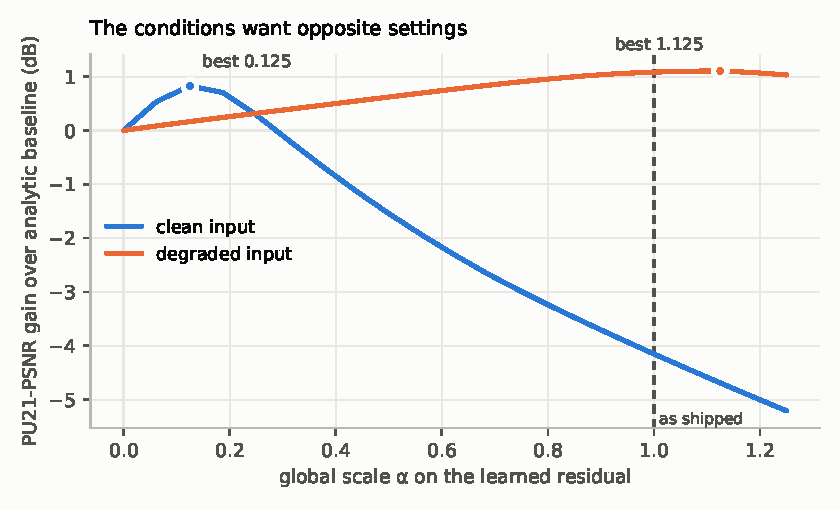
\includegraphics[width=\linewidth]{fig2_alpha_sweep.pdf}
\caption{Mean gain as a function of the global residual scale $\alpha$. The
curves cross: every $\alpha$ that helps one condition hurts the other, and the
shipped $\alpha = 1$ is near-optimal for degraded input and near-worst for
clean.}
\label{fig:alpha}
\end{figure}

The two conditions want opposite settings. Clean improves monotonically as
$\alpha$ falls to $\approx 0.125$, hard as it rises to $\approx 1.1$, and no
constant serves both: the constant that repairs clean discards 85\% of the
degraded-input gain. Per-frame adaptation beats the shipped configuration by
\SI{5.84}{\decibel} on clean and \SI{0.29}{\decibel} on hard simultaneously.

The oracle's choice is also legible (\cref{tab:oracle-alpha}). On clean input it
is near-binary in headroom; on degraded input it wants full strength regardless,
because degradation destroys information the baseline cannot recover whatever
the scene's range. A gate would need to see headroom \emph{and} condition
together.

\begin{table}[htbp]
\centering
\caption{Median oracle $\alpha$, split by reference peak.}
\label{tab:oracle-alpha}
\begin{tabular}{lrr}
\toprule
 & peak $<$ \SI{1000}{\nits} & $\ge$ \SI{1000}{\nits} \\
\midrule
clean & \textbf{0.125} & 0.969 \\
hard  & 1.250 & 1.094 \\
\bottomrule
\end{tabular}
\end{table}

\subsection{The ceiling}
\label{sec:ceiling}

We built that gate, a pooled-feature head predicting $\alpha$
(\num{21121} parameters), and trained it three times: twice through the
reconstruction loss, \num{16000} steps in total, and once by direct supervision
on the oracle. All three produced a near-constant output. The trained head emits
$\alpha \in [\num{1.0125}, \num{1.0802}]$ with correlation $-0.037$ against
$\log_2$ of the reference peak, where the oracle wanted \num{0.125}.

Rather than attempt a fourth variant we measured the ceiling directly. On 51
held-out frames, each clean and degraded, giving 102 samples, we fit a linear
readout on exactly the features the head receives, cross-validated \emph{by
frame} so that a clean/degraded pair can never straddle the split
(\cref{tab:ceiling}).

\begin{table}[htbp]
\centering
\caption{Predicting the oracle $\alpha$ from what the gate can see.
Frame-grouped cross-validation, 102 samples.}
\label{tab:ceiling}
\begin{tabular}{lrr}
\toprule
knowing & MAE on oracle $\alpha$ & $R^2$ \\
\midrule
nothing (predict the mean)          & 0.501 & 0.000 \\
the features, via a linear readout  & 0.487 & \textbf{$+0.031$} \\
the condition, \emph{perfectly}     & 0.409 & \textbf{$+0.213$} \\
the oracle itself                   & 0.000 & 1.000 \\
\bottomrule
\end{tabular}
\end{table}

Two numbers close the question. The features explain 3\% of the target's
variance. And 79\% of that variance is \emph{within} a condition and only 21\%
\emph{between} (clean $\alpha$: mean \num{0.436}, sd \num{0.471}; degraded: mean
\num{0.925}, sd \num{0.469}), so a perfect clean-versus-degraded classifier,
which is the most any condition-detection architecture could buy, is capped at
$R^2 = \num{0.213}$. Since 55\% of frames want $\alpha$ at one end of the grid,
the target is close to a binary decision per frame.

The remaining 79\% asks whether \emph{this} frame's clipped region was a
\SI{200}{\nits} lamp or a \SI{20000}{\nits} sun, which is a question about
scene radiance that the delivery frame may not settle.

\paragraph{What this does and does not establish.} It is worth separating the
two, because the temptation to state the stronger version is exactly the error
\cref{sec:corrections} records us making twice already.

\emph{Established.} The variance decomposition is a property of the oracle
target and the condition labels, not of any model: 79\% of the variance in
$\alpha$ lies within a condition, so no architecture that works by detecting the
condition, however good, can explain more than $R^2 = \num{0.213}$. That ceiling
is real and holds for any method of that shape.

\emph{Measured, but of one representation.} The $3\%$ figure is what a
\emph{linear} readout of the pooled features \emph{this particular head sees}
recovers, on 102 samples from 51 frames. It bounds that readout and that
representation. It does not bound what some other representation might hold: the
signal could be nonlinear in these features, or spatial where these are pooled,
or semantic, or present in the frame and absent from anything we extracted.

\emph{Not established.} That the information is absent from the 8-bit frame. We
varied capacity, corpus and objective by a factor of four to six
(\cref{sec:levers}) and nothing moved, which is evidence against a trivial
architecture fix and is not a proof of unidentifiability. A formal statement
would need a bound we have not derived. What we claim is the empirical version:
\emph{the oracle scale is poorly identifiable from the single-frame
representations we tested}, and the \SI{5.84}{\decibel} it is worth stayed out
of reach of every attempt we made to predict it.

\paragraph{What \emph{is} detectable.} The one axis that carries signal is the
condition itself. A frame-grouped cross-validated classifier on the same
features reaches \textbf{75.5\%} accuracy at separating clean from degraded,
against 3\% of the variance explained for the continuous target. That asymmetry
is the whole opening, and \cref{sec:gate} walks through it.

\subsection{Three levers, one bound}
\label{sec:levers}

The bound is not an artefact of any one design choice. Each of the three levers
usually reached for was varied by a factor of four to six (\cref{tab:levers}).

\begin{table}[htbp]
\centering
\caption{None of the three standard levers moves the bound.}
\label{tab:levers}
\begin{tabular}{lll}
\toprule
lever varied & change & effect \\
\midrule
capacity  & \num{1.20}M $\rightarrow$ \num{4.77}M parameters & $\pm$\SI{0.5}{\decibel}, sign varies (\cref{sec:capacity}) \\
corpus    & $6\times$ footage & \SI{+0.03}{\decibel} \\
objective & censored loss; oracle supervision & no movement in $\alpha$ \\
\bottomrule
\end{tabular}
\end{table}

\section{The shadow gate: reaching the reachable part of the bound}
\label{sec:gate}

\subsection{Reformulating the question}
\label{sec:reformulation}

\Cref{sec:bound} asks a hard question: predict a continuous per-frame scale, of
which only 21\% of the variance is explained by the clean/degraded distinction
and only 3\% by the available features. \Cref{sec:ablation} makes a different
question available. The shadow arm is a \emph{binary} decision, and its correct
setting is \emph{exactly} the clean-versus-degraded axis, which is the part that
is partially detectable at 75.5\%.

The consequence is arithmetic. At that measured accuracy, a switch on the shadow
arm alone is worth \SI{+2.65}{\decibel} of clean for \SI{0.27}{\decibel} of hard
(\cref{tab:prediction}). That was the prediction we set out to test.

\begin{table}[htbp]
\centering
\caption{Predicted value of a switch on the shadow arm at the measured 75.5\%
classifier accuracy, against the shipped configuration.}
\label{tab:prediction}
\begin{tabular}{lrr}
\toprule
 & clean & hard \\
\midrule
shipped                      & \SI{-3.00}{\decibel} & \SI{+1.43}{\decibel} \\
75.5\%-accurate arm switch   & \textbf{\SI{-0.35}{\decibel}} & \textbf{\SI{+1.16}{\decibel}} \\
\bottomrule
\end{tabular}
\end{table}

\subsection{The gate, trained}
\label{sec:gate-trained}

\textsc{ShadowGate} is \num{21121} parameters on the frozen v5 backbone,
predicting the single weight $\sw$ of \cref{eq:prior} per frame. By construction
$\sw = 1$ reproduces the shipped configuration exactly and $\sw = 0$ reproduces
the ablated configuration exactly, so it interpolates between the two measured
endpoints of \cref{tab:ablation} and nothing else. It is supervised by binary
cross-entropy against the degradation label, and unlike the residual scale of
\cref{sec:bound} that target needs no oracle: at training time we know whether
we degraded the frame.

\begin{table}[htbp]
\centering
\caption{Gain over the analytic baseline, 429 held-out frames. The gated
configuration is the only row that is positive on all four measures.}
\label{tab:gate}
\begin{tabular}{lrrrr}
\toprule
method & clean dB & clean JOD & hard dB & hard JOD \\
\midrule
v5, as shipped            & $-3.00$ & $-0.046$ & \textbf{$+1.43$} & \textbf{$+0.443$} \\
v5, shadow arm off        & $+0.51$ & $-0.017$ & $+0.33$ & $+0.134$ \\
v6, $4\times$ capacity    & $-2.75$ & $+0.004$ & $+0.96$ & $+0.344$ \\
\textbf{v5 + shadow gate} & \textbf{$+0.07$} & \textbf{$+0.113$} & \textbf{$+1.24$} & \textbf{$+0.389$} \\
\bottomrule
\end{tabular}
\end{table}

The gate beat the prediction on both axes: predicted \SI{-0.35}{\decibel} clean
and \SI{+1.16}{\decibel} hard, delivered $+0.07$ and $+1.24$ on the first seed
(\cref{tab:gate}) and $+0.41 \pm 0.33$ and $+1.12 \pm 0.15$ across three
(\cref{sec:seeds}). Against the shipped model that is
$+3.41 \pm 0.32$~dB and $+0.135 \pm 0.023$~JOD on clean for
$0.30 \pm 0.15$~dB and $0.091 \pm 0.041$~JOD on hard: it converts the
clean regression into a win while keeping most of the degraded-input gain.

Two properties deserve stating precisely. First, it is the only configuration we
scored that is positive on all four measures; every other row buys one column
with another. Second, its clean CVVDP of \num{9.561} exceeds \emph{both ends of
the ablation it interpolates} (\num{9.402} with the arm on, \num{9.431} with it
off) and every fixed alternative including the $4\times$ capacity model. A hard
switch could not do that. The gate is emitting intermediate weights and finding
per-frame settings that neither extreme reaches, which is more than the binary
framing that motivated it predicted.

\subsection{Three seeds}
\label{sec:seeds}

The \SI{+0.07}{\decibel} clean margin above is small enough that one run proves
nothing, so we trained two further gates on the same backbone, changing only the
seed, and scored them on the same 429 frames (\cref{tab:seeds}).

\begin{table}[htbp]
\centering
\caption{Three gate seeds, gain over the analytic baseline. CVVDP and frames won
are on clean, out of 429; the shipped v5 wins 115 for comparison.}
\label{tab:seeds}
\setlength{\tabcolsep}{4.5pt}
\begin{tabular}{lrrrrrr}
\toprule
 & \multicolumn{2}{c}{clean} & \multicolumn{2}{c}{hard} & clean & clean \\
\cmidrule(lr){2-3}\cmidrule(lr){4-5}
seed & dB & JOD & dB & JOD & CVVDP & frames won \\
\midrule
\num{20260901} & $+0.07$ & $+0.113$ & $+1.24$ & $+0.389$ & 9.561 & 251 (59\%) \\
2              & $+0.71$ & $+0.068$ & $+0.96$ & $+0.308$ & 9.516 & 315 (73\%) \\
3              & $+0.45$ & $+0.089$ & $+1.18$ & $+0.358$ & 9.537 & 280 (65\%) \\
\midrule
\textbf{mean $\pm$ sd} & \bm{$+0.41$} & \bm{$+0.090$} & \bm{$+1.12$} & \bm{$+0.352$} & & \\
 & \bm{$\pm 0.33$} & \bm{$\pm 0.023$} & \bm{$\pm 0.15$} & \bm{$\pm 0.041$} & & \\
\bottomrule
\end{tabular}
\end{table}

All three seeds are positive on all four measures, and all three reach a clean
CVVDP above every fixed alternative we scored (best of those: \num{9.452}). The
result is a property of the method rather than of a seed.

It is worth recording which way the single-run report erred. Seed
\num{20260901} is the \emph{worst} of the three on clean PU21 ($+0.07$ against a
mean of $+0.41$) and the \emph{best} on clean CVVDP ($+0.113$ against
$+0.090$). Reporting it alone understated the decibel result by a factor of six
and overstated the JOD result by a quarter. The honest headline is the mean with
its spread, and that is what the abstract carries.

\subsection{An observation about the selection criterion}
\label{sec:selection-observation}

Each gate's checkpoint is chosen by a trailing median over
degradation-classification accuracy on validation: 69.5\%, 64.1\% and 64.8\% for
seeds \num{20260901}, 2 and 3. Ranked by that accuracy, the three runs come out
in exactly the order of their clean CVVDP and in exactly the reverse order of
their clean PU21 (\cref{tab:rank}).

\begin{table}[htbp]
\centering
\caption{Validation classification accuracy against clean-condition outcome,
three seeds. With $n = 3$, a perfect agreement or inversion arises by chance
with $p = 1/6$; this is an observation, not a result.}
\label{tab:rank}
\begin{tabular}{lrrrrrr}
\toprule
seed & val accuracy & rank & clean JOD & rank & clean dB & rank \\
\midrule
\num{20260901} & 69.5\% & 1 & $+0.113$ & 1 & $+0.07$ & 3 \\
3              & 64.8\% & 2 & $+0.089$ & 2 & $+0.45$ & 2 \\
2              & 64.1\% & 3 & $+0.068$ & 3 & $+0.71$ & 1 \\
\bottomrule
\end{tabular}
\end{table}

We report it because it is the disagreement of \cref{sec:disagreement} appearing
a third time, after the metrics themselves and after the selection rule of
\cref{sec:selection}, now in a criterion that touches neither metric. Whatever
the gate learns that makes a frame classifiable also makes it look better and
measure worse. Three seeds cannot settle that; it is the first thing we would
test with thirty.

\section{Evaluation methodology: three defects in our own harness}
\label{sec:methodology}

We report these because each silently corrupted a result we believed, and each
is a mistake available to any comparable pipeline.

\subsection{Selection on a maximum over noise}
\label{sec:selection}

The shipped checkpoint was chosen by the \emph{maximum} of the composite
criterion
\begin{equation}
\texttt{composite\_gain} \;=\; \texttt{hard\_gain} + \min\!\big(0,\ \texttt{clean\_gain}\big)
\label{eq:composite-gain}
\end{equation}
over 102 in-training evaluations. Across that run \texttt{clean\_gain} had mean
\SI{-1.43}{\decibel} and standard deviation \SI{1.29}{\decibel}, with only 10 of
102 evaluations positive; the shipped checkpoint's $+0.02$ ranked 9th of 102.
Its promised hard gain of \SI{+1.80}{\decibel} measured \SI{+1.43}{\decibel} on
held-out frames, between the evaluation mean ($+1.19$) and its selected maximum,
which is exactly where an inflated in-training figure should land. Selection now
uses a trailing median over five evaluations; replayed on the same series it
selects step \num{72000} instead of \num{81000}.

We then scored step \num{72000} on the same 429 frames, and the answer is not
the clean vindication we expected. On the criterion the selector optimises it is
better: composite gain \SI{-1.36}{\decibel} against the shipped checkpoint's
\SI{-1.57}{\decibel}, and clean PU21 improves by \SI{+0.55}{\decibel}. On CVVDP
it is \emph{worse on both conditions}, $-0.052$~JOD clean and $-0.071$~JOD hard,
so the smoothed rule would have shipped a checkpoint that a perceptual metric
likes less. This is the disagreement of \cref{sec:disagreement} reappearing
inside the selection rule itself: median smoothing removes the noise it was
designed to remove, and the objective it smooths is still PU21. Smoothing a
selector does not fix choosing the wrong quantity to select on. We report the
fix and its limit together, because reporting only the first would repeat the
error this section is about.

\subsection{An evaluation that read the front of the split}
\label{sec:front-of-split}

\texttt{DataLoader(val, shuffle=False)} with \texttt{max\_batches=N} evaluates
the alphabetically \emph{first} $N$ records: 32 records across 11 scenes, every
name between \texttt{abandoned\_factory} and \texttt{blau\_river}, with 403
records and 87 scenes never measured. Since error correlates with headroom
(\cref{sec:headroom}), that slice reported a clean gain of $+0.61$ where the
benchmark measures $-3.0$. Fixed with a seeded permutation applied identically
to both conditions.

\subsection{A viewer that presented every frame upside down}
\label{sec:flip}

The default framebuffer places row 0 at the bottom and the display shader
sampled its texture coordinate unchanged. No numeric test caught it, because
they all compare the float composite, which a presentation flip leaves
untouched, and the one test that read the canvas did so through
\texttt{readPixels}, which returns rows bottom-first and cancelled the flip
against itself. Master EXR output was never affected.

\subsection{Two claims we corrected against fresh measurement}
\label{sec:corrections}

\Cref{sec:tail} has been rewritten twice against new measurements. The first
draft claimed the model invents highlights; the second claimed the penalty was
tail-carried. Both were wrong, and both were plausible. We record this beside
the harness defects because the mechanism is the same: a hypothesis that
explains the headline number is not thereby established, and in both cases the
measurement that settled it was cheap.

\section{Limitations}
\label{sec:limitations}

\paragraph{Held-out size.} 429 test frames over 97 scenes. The oracle and
ceiling analyses of \cref{sec:bound} use 27 and 51 frames respectively, one per
scene; that sample runs approximately \SI{1.15}{\decibel} pessimistic on clean
against the full set (\SI{-4.15}{\decibel} at $\alpha = 1$ where the full 429
read \SI{-3.00}{\decibel}). Ordering is reliable; absolute values will move.

\paragraph{Distribution shift.} The train/test shift of \cref{sec:shift} is a
confound in the clean result. \Cref{sec:ceiling} argues it is not the binding
constraint, but we have not retrained under a matched sampler to prove it.

\paragraph{The oracle is an upper bound.} It reads the ground truth.

\paragraph{Single-image only.} The temporal refiner is not evaluated here; its
held-out set is 4 validation and 5 test clips of one scene each, too small to
report.

\paragraph{The analytic baseline is privileged on clean corpus frames.}
\Cref{eq:baseline} is the exact inverse of the transform that rendered the
corpus SDR side, so on clean frames it is being handed the forward pipeline. It
is an unusually strong control, which is what makes the comparison sharp, and it
is also unusually strong in a way no baseline would be on footage from elsewhere.
A clean-condition regression against it should be read as ``worse than knowing
the exact forward transform'', not as a general statement about learned inverse
tone mapping against whatever baseline a real pipeline would have. The degraded
condition does not have this property, since no analytic inverse knows the
degradation.

\paragraph{One degradation model, and a gate supervised on it.} \textsc{hard}
is our own seeded camera and codec pipeline, not a corpus of real degraded
footage. This bears harder on the gate than on the model: the gate is trained by
binary cross-entropy against \emph{our} degradation label, so what it learns may
be the signature of this generator, JPEG blocking, 4:2:0 chroma, the particular
banding and tone-curve family, rather than the property we want, which is that a
frame's shadows need reconstruction. Nothing in our evaluation separates the
two, because the test condition is generated the same way as the training
condition. The experiment that would separate them is to hold out a degradation
family entirely, train on the rest and test on it, and better still to score
real degraded footage that our pipeline never touched. Until that is run, the
gate's 75.5\% should be read as accuracy on this degradation model.

\paragraph{One published method, not four.} ExpandNet is scored on our split
(\cref{sec:expandnet}); Santos et al., Eilertsen et al.~and Liu et al.~have
public code and are not. One comparison answers ``compared to what?'' and does
not rank the field, and the caveats of \cref{sec:expandnet}, namely
training-domain mismatch, an unclamped reference and a per-frame exposure fit,
apply to the one row we have.

\paragraph{No claim here rests on a reimplementation of prior work.}
\Cref{sec:related} places the result among families of methods and cites them
bibliographically; it does not reproduce their numbers, and we did not run their
code.

\paragraph{Three seeds is a spread, not a distribution.} The gate is positive on
all four measures in all three runs, but $n = 3$ supports ``the sign is stable'',
not a confidence interval. The clean PU21 spread ($+0.07$ to $+0.71$) is wide
relative to its mean.

\paragraph{Deployment carries the gate as a scalar only.} The interactive viewer
receives the predicted shadow weight per frame and multiplies the shadow prior
by it in the compositing shader; CPU/GPU parity holds to
$8.4 \times 10^{-6}$ relative error across 11 cases spanning $\sw = 0$ to
$\sw = 1$. The weight cannot be folded into the residual the way a scalar
residual scale can, because it enters inside the $\max$ of \cref{eq:prior} and
is not linear in the residual.

\section{Conclusion}
\label{sec:conclusion}

A \num{1.2}M-parameter residual on an analytic inverse tone map is worth
\SI{+1.43}{\decibel} and $+0.44$~JOD on degraded input, on 81\% of held-out
frames, and costs \SI{3.0}{\decibel} of PU21-PSNR on clean input for a
perceptually invisible $-0.046$~JOD. Its defect is that it does not know when to
do nothing.

We measured what repairing that is worth, an oracle per-frame scale being
\SI{+5.84}{\decibel} on clean, and then measured how much of that scale is
predictable from what the model can see. A linear readout of the features the
gate receives explains 3\% of its variance, and 79\% of the variance lies within
a condition rather than between, so even a perfect clean-versus-degraded
classifier is capped at $R^2 = \num{0.213}$. Capacity, corpus and objective were
each varied by a factor of four to six; none moved it. The ceiling on
condition-detection is a property of the target and holds for any architecture
of that shape; the 3\% is a statement about one representation and one linear
readout, and we do not claim to have shown the information is absent from the
frame.

The bound is a property of the question. Asked for a continuous scale, the input
cannot answer. Asked a binary question on the axis that \emph{is} detectable,
whether this frame arrived clean or degraded, it can. Locating the failure in
the shadow arm rather than in the highlights made that decomposition available,
and a \num{21121}-parameter gate on that arm delivers
$+3.41 \pm 0.32$~dB and $+0.135 \pm 0.023$~JOD on clean for
$0.30 \pm 0.15$~dB and $0.091 \pm 0.041$~JOD on hard across three seeds:
the only configuration we scored that is positive on all four measures, in every
run, with a clean CVVDP that exceeds both ends of the ablation it interpolates.

The lesson we would carry to another problem is not about tone mapping. Four of
the things that cost us most in this work were measurement defects rather than
model defects. Three are in \cref{sec:methodology}: selection on the maximum of
a noisy series, an evaluation that read the alphabetical front of its split, and
a viewer that presented every frame upside down beneath tests that only ever
compared float buffers. The fourth is in \cref{sec:seeds}, and is the one we
would warn a reader about first: our initial report of the gate quoted a single
seed that happened to be the weakest of three on one metric and the strongest on
the other. We would not have known without running the other two.

The ceiling we could prove was real, the one we could only measure held against
everything we threw at it, and so were the ways we nearly failed to see either.


\bibliographystyle{plainnat}
\bibliography{refs}

\appendix
\section{Notation}
\label{sec:notation}

\begin{table}[htbp]
\centering
\caption{Symbols used throughout.}
\label{tab:notation}
\begin{tabular}{ll}
\toprule
symbol & meaning \\
\midrule
$\Lsc$ & scene radiance in network units; $1.0 = \SI{10000}{\nits}$ \\
$\sdr$ & 8-bit SDR frame, $[0,1]^{H\times W\times 3}$ \\
$T$ & unknown display-referred transform (exposure, grade, tone curve) \\
$c$ & delivery ceiling of a graded source \\
$\base(\sdr)$ & analytic inverse-tone-map baseline, \cref{eq:baseline} \\
$\resid$ & learned log-domain residual \\
$\hmask, \smask$ & learned highlight and shadow masks \\
$p_{\mathrm{h}}, p_{\mathrm{s}}$ & fixed per-pixel highlight and shadow priors, \cref{eq:prior} \\
$\gate$ & per-pixel residual gate \\
$\sw$ & per-frame shadow-arm weight, predicted by the gate of \cref{sec:gate} \\
$\alpha$ & global scale on the residual, \cref{sec:oracle} \\
$\lscale$ & log encoding scale, $\lscale = 16$ \\
$\maxhdr$ & network output ceiling, $4.0 = \SI{40000}{\nits}$ \\
$\ell(x)$ & $\log(1 + \lscale x)$ \\
\bottomrule
\end{tabular}
\end{table}

\section{Reproducibility}
\label{sec:reproducibility}

The benchmark is four exports and six scorings, resumable:

\begin{Verbatim}[fontsize=\small]
# the full benchmark
powershell -ExecutionPolicy Bypass -File training\run_bench.ps1

# one more checkpoint against the same reference
powershell -ExecutionPolicy Bypass -File training\score_checkpoint.ps1 `
    -Checkpoint <ckpt> -Name <label>

# every derived number in the results sections recomputed from those
# results and diffed against the paper; exit status 1 on any mismatch
python training\audit_paper_numbers.py --bench <bench dir>

# the headroom split and its correlation, from the same results joined
# to the corpus manifest's per-frame peak luminance
python training\analyze_headroom.py --bench <bench dir> `
    --manifest <manifest> --check
\end{Verbatim}

Results land as a results document, per-clip JSON and per-frame CSV. The
composite of \cref{eq:composite} exists in three languages, PyTorch, GLSL and
NumPy, pinned against each other to $8.4 \times 10^{-6}$ relative error by a
parity test. The test suite covers those, canvas orientation
(\cref{sec:flip}), PU21 torch-versus-numpy parity, and a smoke test that
exercises all 54 controls of the interactive viewer.

The audits above are not decoration. An earlier draft reported 346 of 429 frames
won on degraded input where the benchmark says 348; the count had been
transcribed by hand, and nothing in the pipeline compared it back to the file it
came from. An earlier draft gave v6 \num{4772485} parameters where the
checkpoint has \num{4770117}, for the same reason. Every derived number in
\cref{sec:results,sec:failure,sec:gate} is now recomputed on demand, and both
scripts exit non-zero on any drift.

Two analyses remain uncovered by that audit: the trimmed-PSNR table of
\cref{sec:tail} and the oracle sweep of \cref{sec:oracle}. Both need per-pixel
statistics over the reference frames rather than the per-frame results the
benchmark writes, and we state that rather than leaving a reader to assume
otherwise.

Weights, frame pairs and HDR sources are not distributed; the training scripts
regenerate them.

\section{Standards referenced by the pipeline}
\label{sec:standards}

\begin{itemize}
\item SMPTE ST 2084:2014, the PQ electro-optical transfer function of mastering
  reference displays \citep{st2084}.
\item ITU-R BT.2100, image parameter values for high dynamic range television
  \citep{bt2100}.
\item ITU-R BT.2408, operational practices in HDR television production, from
  which diffuse white at \SI{203}{\nits} is taken \citep{bt2408}.
\item SMPTE ST 2065-4:2013, the ACES image container file layout, AP0
  chromaticities \citep{st20654}.
\end{itemize}

\section{Relation to an earlier manuscript}
\label{sec:withdrawal}

An earlier manuscript from this group described a DRE-transformer and
cross-attention architecture and reported results for it. Two things in that
document are withdrawn without qualification.

First, its results tables quoted an ``HDR-VDP-3'' column that corresponds to no
metric this codebase ever computed. The only HDR perceptual metric implemented
is ColorVideoVDP, which reports JOD on a roughly 0 to 10 scale. Those tables
were placeholders and should never have been presented as measurements.

Second, the architecture those tables described was never trained to
completion, so rows implying an evaluated system were aspirational.

The present paper reports a different system: a direct SDR-pixel to
scene-linear-radiance image model, measured with the metrics that exist. We
record the withdrawal here rather than silently omitting it, because a reader
who has seen the earlier document is entitled to know which claims were retired
and why. The caution about citations at the head of \cref{sec:related}, and the
audit scripts of \cref{sec:reproducibility}, are both direct responses to that
failure.


\end{document}
